\chapter{Premilinaries and Problem Definition}
\label{ch:premAndDef}


\section{The Friedkin and Johnsen Model}
\label{sec:prem}

The Friedkin-Johnsen model is a very popular extension of the DeGroot's model. This model uses information about the opinion of the user assuming there is an internal and external opinion. The internal opinions cannot change and is the specific opinion of an individual for a certain matter. On the other hand the expressed opinion is influenced by social interactions.
\\
\\
The expressed opinion of a user is computed as a weighted average of the external opinions of the neighbourhood of the user, for example, the opinions of the users friend list or the accounts the user follows.
\\
\\
The opinions of the users are stored in a vector. This vector is a metric for the whole social graph and can give us insights about its current situation. 
\clearpage


\noindent The vector values range from [-1,1]. Values closer to the range limits indicate bigger polarization. Polarized graphs create groups of nodes that are strongly connected with each other.
\\
\\
\noindent Let $G = (V,E)$ be a connected undirected graph representing a network. Let $z$ be the vector of expressed opinions  for the whole network. Each value  of the vector represents a node and can be computed with the opinion-formation model of Friedkin and Johnsen as follows. 

\begin{equation} 
	z_i = \frac{w_{ii}*si + \sum_{j \epsilon N(i) }{w_{ij}*z_j}} {w_{ii} + \sum_{j \epsilon N(i) }{w_{ij}}} 
\end{equation} 
\\

\noindent Where $s_i$ denotes the internal and $z_i$ the expressed opinion of a user. The internal opinion of a user corresponds to the views that inherently holds for a controversial topic while the expressed refers to the views that the user shares on a social network with his friends. 
\\
\\
The length of the opinion vector $||z|| ^2$ measures  the polarization of the network. To make the polarization  independent of its network we can  normalize it  by dividing  it with the length of the vector $z$. 
\\
\\
An equivalent way of obtaining the vector $z$ from a graph is the following: if $L$ is the laplacian matrix of a graph $G=(V,E)$, and $I$ is the identity matrix, then $z=(L+I)^{-1}S$ \cite{bindel}. 

\section{Measuring the polarization}
\label{sec:meas}

\noindent We use the definition of the polarization index by Matakos et al. The polarization is measured by its distance from a neutral opinion. 
\\
\\
We can quantify this with the length of the vector of the second norm $L_{2}^2$ \cite{tsapMatakosTerzi}.
\clearpage


\begin{equation}
	\pi(z) = ||z||_{2}^2
\end{equation}
\\
This value can be independent of the network if we normalize it by dividing with the size of the graph.

\section{Problem Definition}
\label{sec:problemDef}

\noindent Let $G = (V,E)$ be a connected undirected graph representing a network. Let $z$ be the vector of expressed opinions  for the whole network and $\pi(z) = ||z||_{2}^2$ the polarization index of this social graph.
\\
\\
\noindent Problem 1 [k-Addition]. Let $C \subseteq	V \times V$ a set of edges that are not in the graph. We want to find a subset of $S \subseteq C$ of $k$ edges whose addition to a graph $G$ leads to the greatest reduction of $\pi(z)$.


\subsection{Including probabilities into the problem}
\label{sec:probabilityProbDef}

Problem 1 is trying to find edges that will minimize the polarization index. We must not take for granted that these edges will be accepted. 
For example a social media user could reject a new follow/friend request. This leads us to consider additions with the expectation of being accepted. 
\\
\\
The expected polarization can be defined as follows.
\\
\\
\begin{equation}
	E[\pi(z)]= P(u,v) * Val
\end{equation}
\\
\noindent Where $P(u,v)$ is the probabilty of $u$ and $v$ forming an edge and $Val$ is a value specific to our heuristic algorithms. For example $Val$ can be the polarization decrease after the edge addition of $u$ and $v$ or the absolute distance of their opinions.
\clearpage


\noindent Problem 2 [K-Addition-Expected]. Given a graph $G=(V,E)$ and an integer $k$, we want to find a set of $k$ edges $E′ \subseteq V×V \ E$ that when added to $G$ creates a new graph $G' = (V,E \cap E')$ so that the expected polarization score $E[\pi(z)]$ is minimized.


\section{Monotonicity of the Problem}
\label{sec:monotonicity}
\vspace{20pt}
We observe that $\pi(z)$ is not monotone with respect to the edge additions. This means that adding an edge will not necessarily decrease the polarization index. 
\\
\begin{lemma}
The polarization index does not necessarily decrease after an edge addition between opposing views.
\end{lemma}

\vspace{20pt}
\noindent We will  show this with a counter example. In the network~\ref{fig:p5} nodes 0, 2 and 3 have a value of $s_i=-1$, and nodes 2 and 4 have a value of $s_i=+1$. For both examples we assume that $w_{ii}=w_{ij}=w_{ji}=1$ and $n$ the number of nodes.
\\
\\
We will now compute the polarization index of the original graph
\\
\\
\begin{figure}[h]
	\centering
	\begin{subfigure}[t]{0.3\textwidth}
		\centering
		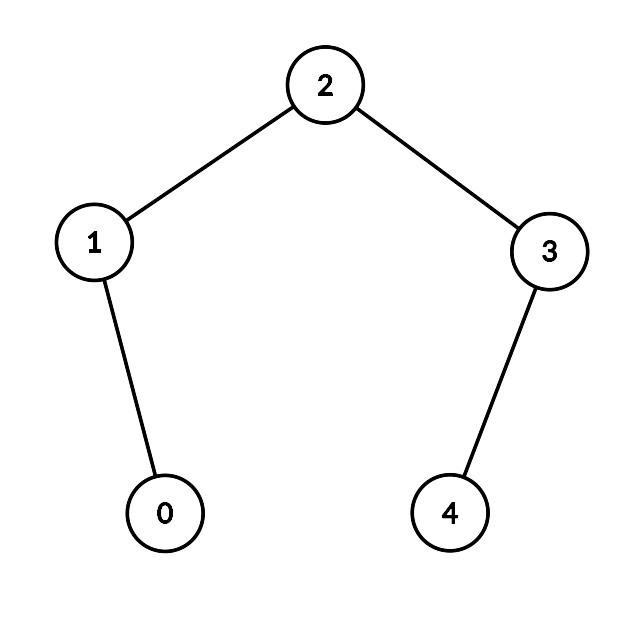
\includegraphics[height=0.15\textheight]{Figures/p5A}
		\caption{}
		\label{subfig:monotonicityA}
	\end{subfigure}
	\hfill
	\begin{subfigure}[t]{0.3\textwidth}
		\centering
		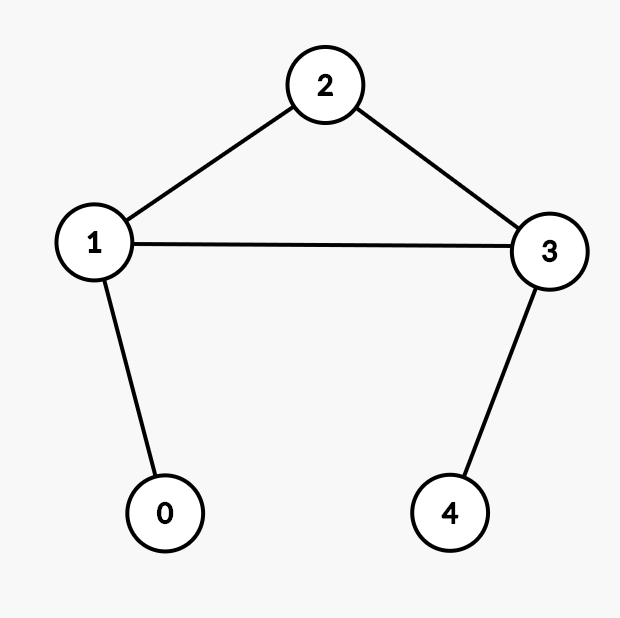
\includegraphics[height=0.15\textheight]{Figures/p5B}
		\caption{}
		\label{subfig:monotonicityB}
	\end{subfigure}
	\vspace{40pt}
	\hfill
	\caption{Edge addition between opposed opinions.}
	\label{fig:p5}
\end{figure}
\\
\\

\clearpage

\begin{equation}
	\begin{aligned}
		(L+I)^{-1}s=z=
		\left(\begin{matrix}
		\frac{-27}{55} \\
		\frac{1}{55} \\
		\frac{-5}{11} \\
		\frac{-21}{55} \\
		\frac{17}{55}
		\end{matrix}\right),
		\qquad \qquad
		\pi(z)= 0.13785123966
	\end{aligned}
\end{equation}
\\
We will now compute the polarization index after the addition of the edge $1\rightarrow3$.

\begin{equation}
	\begin{aligned}
		(L+I)^{-1}s=z=
		\left(\begin{matrix}
		\frac{-53}{99} \\
		\frac{-7}{99} \\
		\frac{-5}{11} \\
		\frac{-29}{99} \\
		\frac{35}{99}
		\end{matrix}\right),
		\qquad \qquad
		\pi(z) = 0.14180185695
	\end{aligned}
\end{equation}
\\
\\
We can see an increase of the polarization index after adding this particular edge. This example was discovered after brute-forcing different graph topologies with different combinations of opinion values.
\clearpage

